\documentclass[12pt]{article}
%\usepackage[utf8]{inputenc}
\usepackage[T1]{fontenc}
\usepackage[latin1]{inputenc}
\usepackage{color}
\usepackage{hyperref}
\usepackage{placeins}
\usepackage{graphicx}
\newcommand\verbbf[1]{\textcolor[rgb]{0,0,1}{\texttt{\textbf{#1}}}}
\newcommand\verbbfb[1]{\textcolor[rgb]{0,0,0}{\texttt{\textbf{#1}}}}

\hypersetup{
  colorlinks,
  citecolor=black,
  filecolor=black,
  linkcolor=black,
  urlcolor=black
}
\usepackage[affil-it]{authblk}

\title{CFIT: Template fits including systematic correlations}
\author{Kirill Skovpen
\thanks{Electronic address: \texttt{kirill.skovpen@cern.ch}}}
\affil{Institut Pluridisciplinaire Hubert Curien, CNRS/IN2P3, Strasbourg, France}
\date{\today}

\begin{document}

\maketitle

\begin{abstract}
CFIT is a tool to perform a template fit with including
systematic uncertainties in a correlation matrix. Systematic
correlations between templates are taken into account. The tool also allows one to estimate
statistical and systematic uncertainties on the fit parameters and to
perform the measurement of the scale factors.
\end{abstract}

\newpage

\tableofcontents

\newpage

\section{Introduction}

Analysis of systematic uncertainties in high energy physics
experiments has always been a place for discussions on realism
and robustness of a chosen approach.
A wide variety of systematic sources ranging from an assessment based on
the first principles to a completely artificial estimation implies a
complexity of statistical description of such uncertainties.
Statistical treatment of asymmetric statistical and systematic
uncertainties in physics analyses is always mentioned as one of the
most obscure and challenging tasks~\cite{BarlowStat,Barlow}.

This paper contains the documentation
of the tool which was developed to perform the Monte Carlo template fit to data by
including systematic uncertainties in the fit via a correlation matrix.
Such methods are widely used in various physics analyses. This
paper does not introduce any novelty in statistical methods used
whilst it attempts to have a specific implementation for a chosen
approach, as well as to adapt several ideas outlined in other papers referenced
here by testing it further in a dedicated tool.

\section{Install}

Here are a few steps to build the shared library for CFIT:

\begin{verbatim}
git clone https://github.com/kskovpen/CFIT
cd CFIT/
make
\end{verbatim}

\section{Fit procedure}

Minimisation is performed in MINUIT~\cite{Minuit} using the following
$\chi^2$ function:

\begin{equation}
\chi^2 = \frac{
(x^{d}_{i}-\sum\limits_{k=1}^{N_{t}}P_{k}x^{k}_{i})
V_{ij}^{-1}
(x^{d}_{j}-\sum\limits_{k=1}^{N_{t}}P_{k}x^{k}_{j})
}
{\sqrt{
(\sigma_{i}^{d})^2 +
(\sum\limits_{k=1}^{N_{t}}\sigma_{i}^{k})^2
}
\sqrt{
(\sigma_{j}^{d})^2 +
(\sum\limits_{k=1}^{N_{t}}\sigma_{j}^{k})^2
}
},
\end{equation}

\noindent where $x^{d}_{i}$ is the number of data events in $i$-bin,
$x^{k}_{i}$ is the number of events for $k$-template in $i$-bin,
$\sigma_{i}^{d}$ is the statistical uncertainty in data in $i$-bin,
$\sigma_{i}^{k}$ --- total uncertainty for $k$-template in $i$-bin,
$N_{t}$ is the number of templates.
$V_{ij}$ is the correlation matrix element which is constructed as follows:

\begin{equation}
V_{ij} = \frac{\sum\limits_{s=1}^{N_{sys}} C_{s}
\sigma_{i}^{s}\sigma_{j}^{s} +
\delta_{ij}\sigma_{i}^{MCstat}\sigma_{j}^{MCstat} +
\delta_{ij}\sigma_{i}^{d}\sigma_{j}^{d}}
{\sqrt{
(\sigma_{i}^{d})^2 +
(\sigma_{i}^{MC})^2
}
\sqrt{
(\sigma_{j}^{d})^2 +
(\sigma_{j}^{MC})^2
}
},
\end{equation}

\noindent where $N_{sys}$ is the number of systematic variations,
$C_{s}$ is the bin-by-bin correlation factor for $s$-systematics,
$\sigma_{i}^{MCstat}$ is the total statistical uncertainty in $i$-bin
for the sum of templates, and $\sigma_{i}^{k}$ is the total
systematic uncertainty for $k$-systematic variation in $i$-bin:

\begin{equation}
\sigma_{i}^{s} = \sqrt{\sum\limits_{k=1}^{N_{t}}(\sigma_{i}^{k})^{2}},
\end{equation}

\noindent and $\sigma_{i}^{MC}$ is the total uncertainty in $i$-bin:

\begin{equation}
\sigma_{i}^{MC} = \sqrt{\sum\limits_{s=1}^{N_{sys}}(\sigma_{i}^{s})^2+(\sigma_{i}^{MCstat})^2}.
\end{equation}

\noindent The bin-by-bin correlation factor for $s$-systematics is
defined as:

\begin{equation}
C = \frac{2}{N_{b}(N_{b}-1)} \sum\limits_{i=1}^{N_{b}-1}
\sum\limits_{j=i+1}^{N_{b}} \frac{|\sigma_{i}^{+}\sigma_{j}^{+} +
\sigma_{i}^{-}\sigma_{j}^{-}|}
{\sqrt{(\sigma_{i}^{+})^{2} + (\sigma_{i}^{-})^{2}}
\sqrt{(\sigma_{j}^{+})^{2} + (\sigma_{j}^{-})^{2}} },
\end{equation}

\noindent where $N_{b}$ is the number of bins in the template, 
$(\sigma^{+})_{i}^{s}$ and $(\sigma^{-})_{i}^{s}$ are
shape systematic uncertainties which correspond to the positive and negative
one sigma shifts for $s$-systematics. 
For one-sided systematic uncertainty $C = 1$ by definition.

As the $\chi^2$ function is defined only for symmetric
uncertainties, systematic variations in the fitted templates are
symmetrized by using the maximum systematic deviation from the nominal
template as the assigned bin systematic uncertainty:

\begin{equation}
\sigma_{i}^{s} = S \cdot \mathrm{max}
\bigg[|\sigma^{+}|_{i}^{s},|\sigma^{-}|_{i}^{s}\bigg],
\end{equation}

\noindent where $S$ is the sign of the
up-one-sigma variation. An alternative approach of approximation of
asymmetric systematic uncertainties by dimidated Gaussian function is
also implemented in this tool~\cite{Barlow}.

Systematic uncertainties on the templates are recalculated after the
first minimization cycle to provide a more realistic
uncertainty estimation in the $\chi^2$ calculation procedure.

To reduce the effect of correlations in the tails of the distributions
of the templates where such effects might be not well evaluated, bins
yielding up to 2\% of the total statistics in the tail are summed up in one bin.

\section{Estimation of the fit uncertainty}

In order to evaluate uncertainties on the fit parameters, the nominal
templates are replaced by statistic (\verbbf{SetStatVariation}) or systematic
(\verbbf{SetSysVariation}) variations in the
shapes. The fit is performed with all uncertainties included in the fit.
The use of correlation matrix computed with the nominal templates in the
measurement of systematic and statistical uncertainties for the fit
parameters has shown the best stability in terms of a convergence of
the fit. 

\section{Scale factor measurement}

CFIT allows one to perform the measurement of selection criteria efficiencies and the
scale factors from the template fit with the assessment of associated systematic and
statistical uncertainties. For this type of measurement a user has to
specify histograms for all events
(\verbbf{AddTemplate},\verbbf{SetData}), events which passed
the <<tag>> requirement (\verbbf{AddTemplateTag},\verbbf{SetDataTag}), and events with has failed
this requirement (\verbbf{AddTemplateUntag},\verbbf{SetDataUntag}).
Systematic and statistical correlations between the
template fits for different selections are
taken into account. The number of bins in templates has to be the same
for a proper correlation treatment between the different types of selection.
The full example is given in Sec.~\ref{sec:exampleSF}.

\section{User method description}

This section lists the functions which could be used in CFIT.

\vspace{0.3cm}

\noindent \verbbf{cfit(std::string name = "")} --- CFIT constructor,
\verbbfb{name} corresponds to the user defined name of the fit variable.

\vspace{0.3cm}

\noindent \verbbf{void Run(std::string option = "")} --- The main function to run the fit
procedure. If option "tag" is specified, the fit is performed with the post-tag templates.

\vspace{0.3cm}

\noindent \verbbf{void SetVerbose(int v)} --- Set verbose level. 
Two options are possible: no printout (0) and debug printout (1).

\vspace{0.3cm}

\noindent \verbbf{void SetMorphing(OPTMORPHMODE optMorphMode=OPTMORPH\_GEOMETRIC,float frac = 1.)} ---
Set the morphing factor (f) for systematics correlations,
\verbbfb{OPTMORPH\_CUTOFF}: $f=0$ for bins with $b_{i}/b_{max} < frac$, 
\verbbfb{OPTMORPH\_GEOMETRIC}: $f=\sqrt{b_{i}b_{j}}/b_{max}$,
\verbbfb{OPTMORPH\_ARITHMETIC}: $f=(b_{i}+b_{j})/(2 b_{max})$,
\verbbfb{OPTMORPH\_FUNC}: $f=b_{i}b_{j}/b_{max}^{2}$, where $b_{i}$ is
the value for $i$-bin, $b_{max}$ is the maximum bin value in the
histogram.

\vspace{0.3cm}

\noindent \verbbf{int GetMorphing()} --- Get the morphing option for
systematics correlations.

\vspace{0.3cm}

\noindent \verbbf{void SetOptimization(OPTMODE optMode=OPT\_NONE)} --- Set
optimization option for systematics treatment. \verbbfb{OPT\_NONE} --- no
optimization is used, \verbbfb{OPT\_MORPH} --- perform the morphing of systematic
correlations according to \verbbfb{OPTMORPHMODE}, \verbbfb{OPT\_SGN} --- ignore
correlations for bins where systematics flip sign or up and down
variations are of the same sign, \verbbfb{OPT\_SIGMA} --- reset
relative bin systematic uncertainties to $\sigma$ =
$\sqrt{\sum\limits_{i}^{}\sigma_{i}^{2}b_{i})/\sum\limits_{i}^{}b_{i}}$
for bins with $\sigma_{i}/\sigma$~<~0.1, where $b_{i}$ and
$\sigma_{i}$ are the value and the relative uncertainty for $i$-bin.
Combination of several optimization options is also possible:
\verbbfb{OPT\_MORPH\_SGN}, \verbbfb{OPT\_MORPH\_SIGMA}, \verbbfb{OPT\_SGN\_SIGMA},
\verbbfb{PT\_MORPH\_SGN\_SIGMA}.

\vspace{0.3cm}

\noindent \verbbf{int GetOptimization()} --- Get optimization option
for systematics treatment.

\vspace{0.3cm}

\noindent \verbbf{void SetCovarianceMode(COVMODE covMode=COV\_MAX)} ---
Method selection to compute the variance. \verbbfb{COV\_MAX}:
symmetrize bin systematic uncertainty by choosing the maximum deviation,
\verbbfb{COV\_BARLOW}: asymmetric systematic uncertainty approximation 
by dimidated Gaussian~\cite{Barlow}.

\vspace{0.3cm}

\noindent \verbbf{int GetCovarianceMode()} --- Get the method option for
covariance computation.

\vspace{0.3cm}

\noindent \verbbf{void ProducePlots(bool produce = 1)} --- Produce plots
with the results of the fit (\verbbfb{result.eps}), 
correlation matrix (\verbbfb{result.eps}), shape comparison for the
templates (\verbbfb{shape.eps}), shapes for fractional systematic
uncertainties before (\verbbfb{sys.eps}) and after
(\verbbfb{sysOptimised.eps}) optimization.

\vspace{0.3cm}

\noindent \verbbf{int GetNDOF()} --- Get the number of degrees of freedom
($N_{dof}$).

\vspace{0.3cm}

\noindent \verbbf{double GetChisq()} --- Return the
minimized $\chi^{2}/N_{dof}$ value from the fit.

\vspace{0.3cm}

\noindent \verbbf{int GetNPar()} --- Get the number of fitted templates.

\vspace{0.3cm}

\noindent \verbbf{double GetPar(int i)} --- Get the fit parameter for
the $i$-template.

\vspace{0.3cm}

\noindent \verbbf{double GetParErr(int i)} --- Get the error of the
fit parameter for the $i$-template.

\vspace{0.3cm}

\noindent \verbbf{void SetInputFile(std::string fin)} --- Set the name
of the input file with histograms.

\vspace{0.3cm}

\noindent \verbbf{void SetData(std::string name)} --- Set the name of
the data histogram.

\vspace{0.3cm}

\noindent \verbbf{void SetDataTag(std::string name)} --- Set the name of
the data histogram for the post-tag fit.

\vspace{0.3cm}

\noindent \verbbf{void SetDataUntag(std::string name)} --- Set the name
of the data histogram for the un-tag selection.

\vspace{0.3cm}

\noindent \verbbf{void AddTemplate(std::string name,std::string
nominalName,int colour)} ---
Add the title and the histogram name for the nominal template.

\vspace{0.3cm}

\noindent \verbbf{void AddTemplateTag(std::string name,std::string
tagName,int colour)} ---
Add the title and the histogram name for the nominal template for the
post-tag fit.

\vspace{0.3cm}

\noindent \verbbf{void AddTemplateUntag(std::string name,std::string
untagName,int colour)} ---
Add the title and the histogram name for the nominal template for the
un-tag selection.

\vspace{0.3cm}

\noindent \verbbf{void GlueTemplates(std::vector<std::string>
nameV,std::string nameMerged = ``merged'',int colour = 46)} ---
Vary templates with the names specified in \verbbfb{nameV}
simultaneously in the fit. These templates are effectively merged into
one template.

\vspace{0.3cm}

\noindent \verbbf{void GlueTemplatesTag(std::vector<std::string>
nameV,std::string nameMerged = ``merged'',int colour = 46)} ---
The same as \verbbf{GlueTemplates} but for the post-tag templates. The
number of merged templates could be different from what is used in
the pre-tag case.

\vspace{0.3cm}

\noindent \verbbf{void SetMatrixOption(std::string option)} ---
Set the write/read option for correlation matrix. \verbbf{"WRITE"}:
write the result matrix to file, \verbbf{"READ"}: read the matrix from
file.

\vspace{0.3cm}

\noindent \verbbf{void SetMatrixName(std::string name = "matrix")} ---
Set the output name for the ROOT file with correlation matrix.

\vspace{0.3cm}

\noindent \verbbf{void SetLegendHeader(std::string name = "")} ---
Set header for the legend of histograms.

\vspace{0.3cm}

\noindent \verbbf{void AddSys(std::string name,std::string upName,std::string downName)} ---
Add templates which correspond to systematic variations.
\verbbfb{name}: systematics name defined by user;
\verbbfb{upName}: histogram name ending for the one sigma up variation, the full
histogram name is nominalName+upName;
\verbbfb{downName}: histogram name ending for
the one sigma down variation, the full histogram name is
nominalName+downName.

\vspace{0.3cm} 

\noindent \verbbf{void SetSysVariation(std::string name)} --- Replace
nominal template histogram by a systematic variation, \verbbfb{name}
has to be either \verbbfb{upName} or \verbbfb{downName}.

\vspace{0.3cm}

\noindent \verbbf{std::string GetSysVariation()} ---
Get systematic variation name.

\vspace{0.3cm}

\noindent \verbbf{void SetStatVariation(int rnd)} ---
Vary nominal template histogram within the statistical uncertainty,
\verbbfb{rnd} is a seed which has to be greater or equal than 666.

\vspace{0.3cm}

\noindent \verbbf{int GetStatVariation()} ---
Get statistical variation name.

\vspace{0.3cm}

\noindent \verbbf{float GetNData()} ---
Get total sum of events in the input data histogram.

\vspace{0.3cm}

\noindent \verbbf{float GetNTemplate(std::string templateName)} ---
Get total sum of weighted events for a given template.

\vspace{0.3cm}

\noindent \verbbf{float GetErrTemplate(std::string templateName)} ---
Get total error for the sum of weighted events for a given template.

\section{Examples}

Several practical examples are located in \verbbfb{examples/} directory and are briefly
described here.

\subsection{Single fit}

The example below shows how to perform a fit to data with three
templates. All templates have two systematic variations, namely,
\verbbfb{SYS1} and \verbbfb{SYS2}. The example is available in
\verbbfb{examples/test.C} which reads histograms from the file test.root located
in the same directory. The code could be run with the command \verbbfb{root
run.C}. Plots with results from the fit are shown in
Fig.~\ref{fig:result}-\ref{fig:matrix}.

\begin{verbatim}
#include "../cfit.h"

void getResults(CFIT::cfit *cf,float *par,float *err);

void test()
{
   gROOT->SetBatch();
   
   gSystem->Load("../libCFIT.so");

   float par[100];
   float err[100];
   
   CFIT::cfit *cf = new CFIT::cfit("Fit variable");
   cf->SetOptimization(OPT_MORPH_SGN_SIGMA);
   cf->SetMorphing(OPTMORPH_GEOMETRIC);
   cf->ProducePlots(1);
   
   cf->SetInputFile("test.root");

   cf->AddSys("SYS1","_sys1_down","_sys1_up");
   cf->AddSys("SYS2","_sys2_down","_sys2_up");

   cf->SetMatrixOption("WRITE");
   
   cf->SetData("h_data");

   cf->AddTemplate("template1","h_mc1",2);
   cf->AddTemplate("template2","h_mc2",3);
   cf->AddTemplate("template3","h_mc3",4);

   cf->Run();
   
   getResults(cf,par,err);
   float chi2 = cf->GetChisq();
   
   std::cout << "chi2=" << chi2 << std::endl;
   for(int i=0;i<3;i++)
     {
       std::cout << par[i] << " +- " << err[i] << std::endl;
     }   

   delete cf;
   
   gApplication->Terminate();
}

void getResults(CFIT::cfit *cf,float *par,float *err)
{   
   float chi2 = cf->GetChisq();
   int nPar = cf->GetNPar();
   for(int i=0;i<nPar;i++)
     {
        par[i] = cf->GetPar(i);
        err[i] = cf->GetParErr(i);	
     }
}
\end{verbatim}

The fit parameters along with its uncertainties are printed in the
output:

\begin{verbatim}
chi2=0.881485
26.7739 +- 1.58475
48.8739 +- 1.73018
41.3997 +- 1.3972
\end{verbatim}

\FloatBarrier

\begin{figure}[hbtp]
\begin{center}
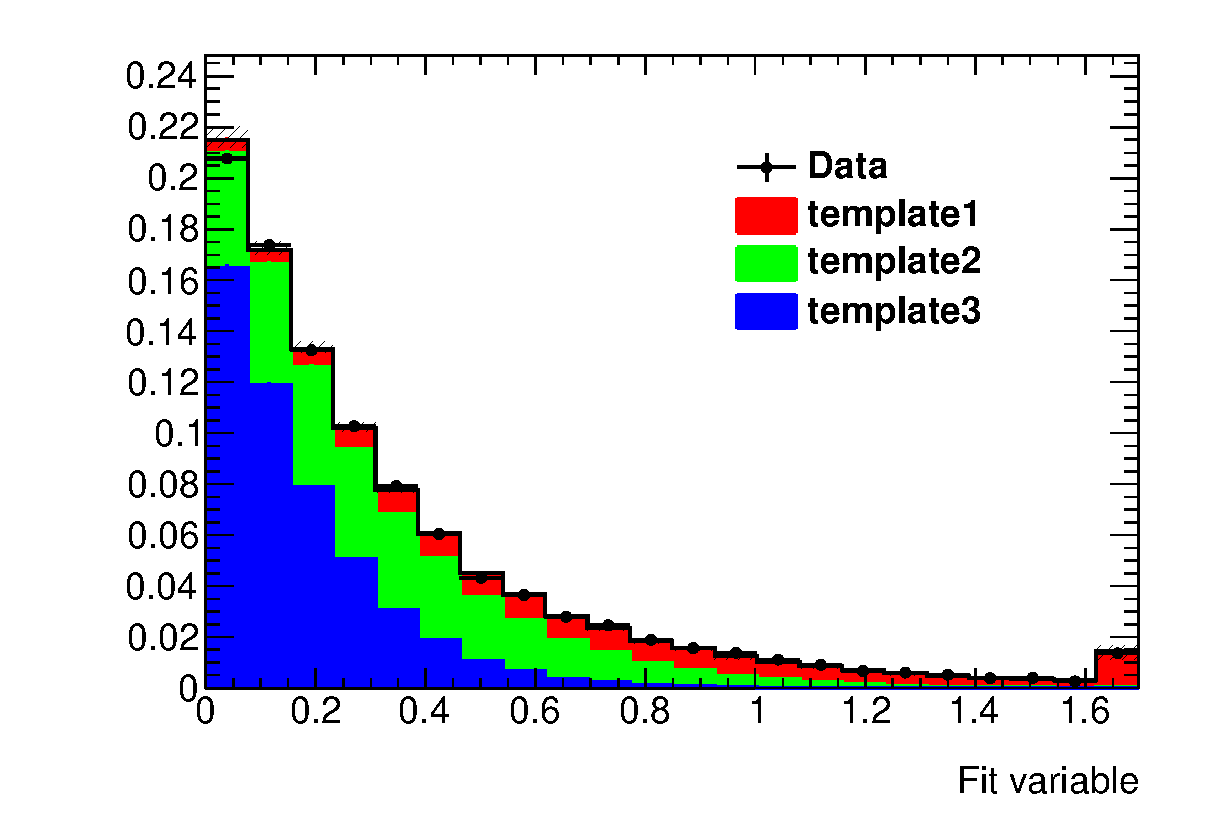
\includegraphics[width=10cm]{pics/result.eps}
\caption{Result of the fit.}
\label{fig:result}
\end{center}
\end{figure}

\begin{figure}[hbtp]
\begin{center}
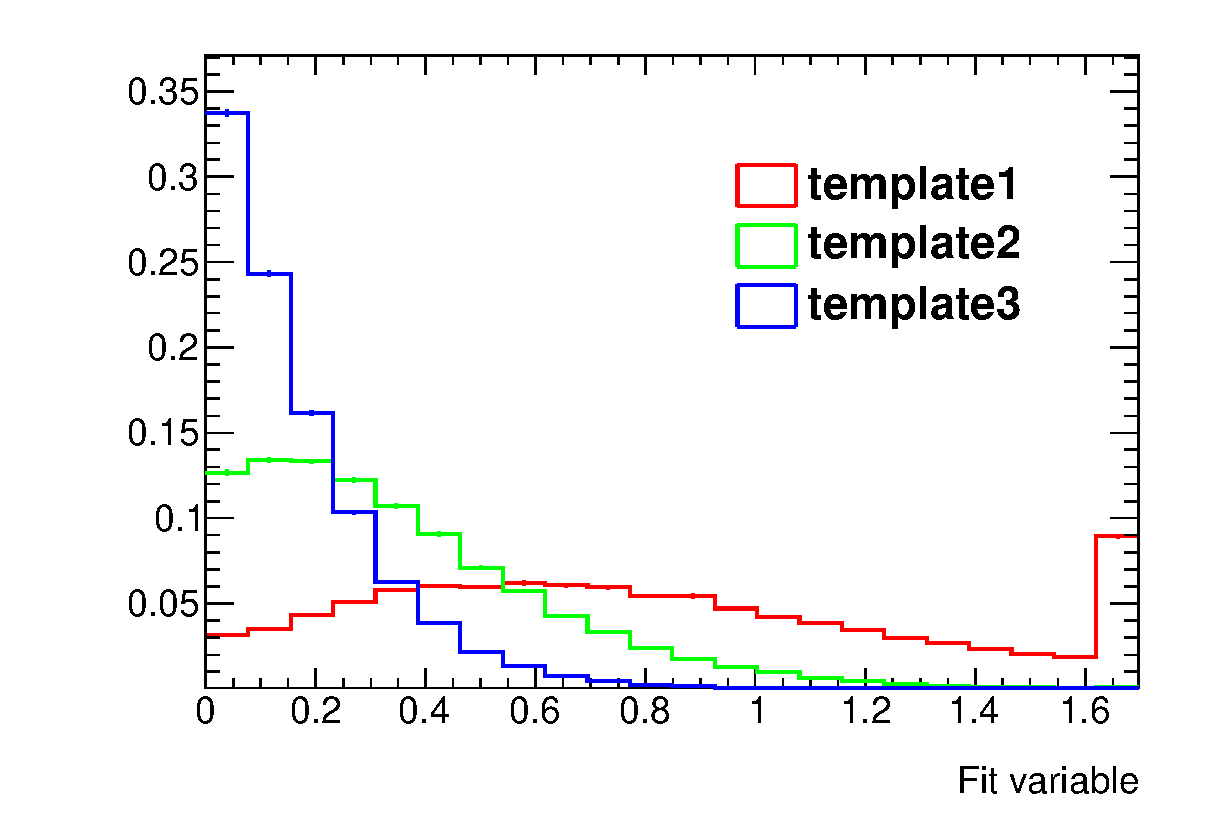
\includegraphics[width=10cm]{pics/shape.eps}
\caption{Shape comparison of the templates.}
\label{fig:shape}
\end{center}
\end{figure}

\begin{figure}[hbtp]
\begin{center}
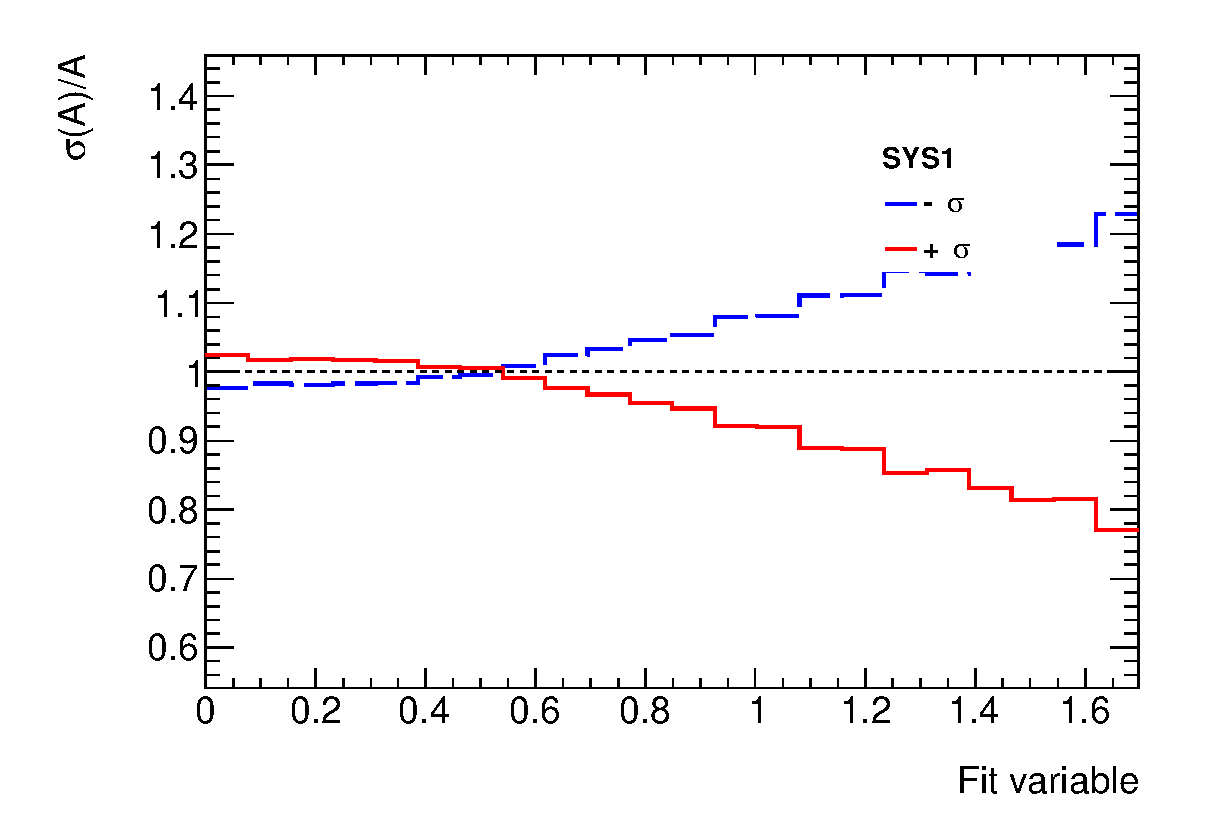
\includegraphics[width=10cm]{pics/sys.eps}
\caption{Fractional systematic uncertainties after optimization
procedure.}
\label{fig:sys}
\end{center}
\end{figure}

\begin{figure}[hbtp]
\begin{center}
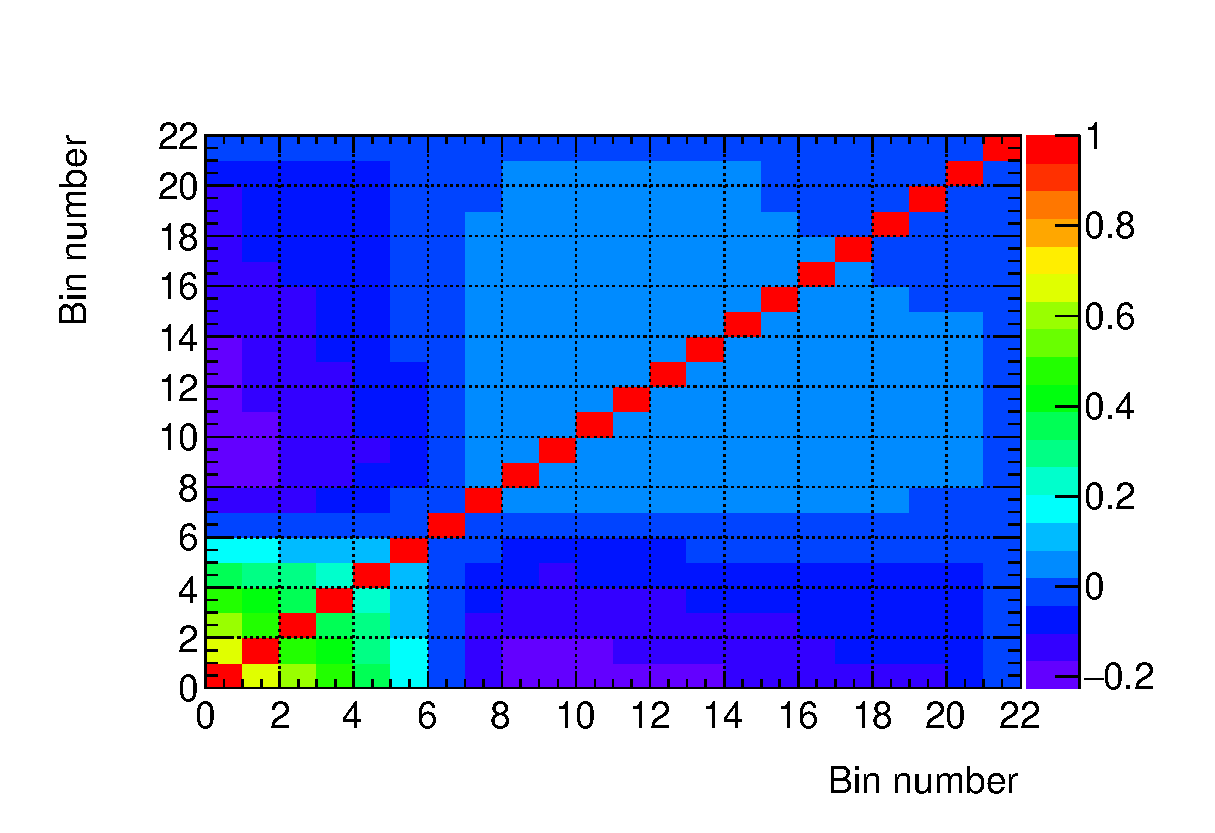
\includegraphics[width=10cm]{pics/matrix.eps}
\caption{Correlation matrix.}
\label{fig:matrix}
\end{center}
\end{figure}

\FloatBarrier

\subsection{Scale factor measurement}
\label{sec:exampleSF}

This example illustrates how to perform the scale factor measurement. The example is available in
\verbbfb{examples/testSF.C} and could be run with the command
\verbbfb{root runSF.C}.

\begin{verbatim}
#include "../cfit.h"

void getResults(CFIT::cfit *cf,float *par,float *err);

void testSF()
{
   gROOT->SetBatch();
   
   gSystem->Load("../libCFIT.so");

   float par[100];
   float err[100];
   float par_tag[100];
   float err_tag[100];
   
   CFIT::cfit *cf = new CFIT::cfit("Fit variable");
   cf->SetOptimization(OPT_MORPH_SGN_SIGMA);
   cf->SetMorphing(OPTMORPH_GEOMETRIC);
   cf->ProducePlots(1);
   
   cf->SetInputFile("test.root");

   cf->AddSys("SYS1","_sys1_down","_sys1_up");
   cf->AddSys("SYS2","_sys2_down","_sys2_up");

   cf->SetMatrixOption("WRITE");
   
   cf->SetData("h_data");
   cf->SetDataTag("h_data_tag");
   cf->SetDataUntag("h_data_untag");
   
   cf->AddTemplate("template1","h_mc1",2);
   cf->AddTemplate("template2","h_mc2",3);
   cf->AddTemplate("template3","h_mc3",4);

   cf->AddTemplateTag("template1","h_mc1_tag",2);
   cf->AddTemplateTag("template2","h_mc2_tag",3);
   cf->AddTemplateTag("template3","h_mc3_tag",4);

   cf->AddTemplateUntag("template1","h_mc1_untag",2);
   cf->AddTemplateUntag("template2","h_mc2_untag",3);
   cf->AddTemplateUntag("template3","h_mc3_untag",4);
   
   cf->Run();   
   getResults(cf,par,err);
   float chi2 = cf->GetChisq();
   float ndata = cf->GetNData();
   float nmc1 = cf->GetNTemplate("template1");
   float nmc = cf->GetNTemplate("template1")+
   cf->GetNTemplate("template2")+
   cf->GetNTemplate("template3");

   cf->Run("tag");   
   getResults(cf,par_tag,err_tag);
   float chi2_tag = cf->GetChisq();
   float ndata_tag = cf->GetNData();
   float nmc1_tag = cf->GetNTemplate("template1");
   float nmc_tag = cf->GetNTemplate("template1")+
   cf->GetNTemplate("template2")+
   cf->GetNTemplate("template3");

   float fr = nmc1/nmc;
   float fr_tag = nmc1_tag/nmc_tag;
   
   float effMC = nmc1_tag/nmc1;
   float effDATA = nmc_tag/nmc*par_tag[0]/par[0]*fr_tag/fr;
   
   std::cout << "effMC = " << effMC << std::endl;
   std::cout << "effDATA = " << effDATA << std::endl;
   std::cout << "sf = " << effDATA/effMC << std::endl;

   // perform statistical variation
   cf->SetMatrixOption("READ");
   cf->SetStatVariation(667);
   cf->ProducePlots(0);   
   cf->Run();
   getResults(cf,par,err);
   cf->SetStatVariation(667);
   cf->Run("tag");
   getResults(cf,par_tag,err_tag);
   
   // do the calculation of SF here again ....
   
   // perform systematic variation
   cf->SetMatrixOption("READ");
   cf->SetSysVariation("_sys1_up");
   cf->Run();
   getResults(cf,par,err);
   cf->SetSysVariation("_sys1_up");
   cf->Run("tag");
   getResults(cf,par_tag,err_tag);
   
   // do the calculation of SF here again ....
   
   delete cf;
   
   gApplication->Terminate();
}

void getResults(CFIT::cfit *cf,float *par,float *err)
{   
   float chi2 = cf->GetChisq();
   int nPar = cf->GetNPar();
   for(int i=0;i<nPar;i++)
     {
        par[i] = cf->GetPar(i);
        err[i] = cf->GetParErr(i);	
     }
}
\end{verbatim}

\begin{thebibliography}{9}

\bibitem{Minuit}
F. James and M. Roos,
Minuit: A System for Function Minimization and Analysis of the
Parameter Errors and Correlations,
Comput. Phys. Commun. 10 (1975) 343.

\bibitem{Barlow}
Roger Barlow, 
Asymmetric Systematic Errors,
\url{arXiv:physics/0306138},
2003.

\bibitem{BarlowStat}
Roger Barlow,
Asymmetric Statistical Errors,
\url{arXiv:physics/0406120},
2004.

\end{thebibliography}

\end{document}
